\documentclass[12pt,a4paper]{article}

\usepackage[a4paper, top = 2cm, bottom = 2cm, left = 1.5cm, right = 1.5cm]{geometry}
\usepackage[dvipsnames]{xcolor} % Colors

\usepackage{standalone}

\usepackage{setspace}
\usepackage{graphicx}
\usepackage{amsfonts}
\usepackage{amsmath}
\usepackage{tikz}
\usepackage{pdfpages}
\usepackage{epigraph}
\usepackage{csquotes}

% Bibliography
\usepackage{xcolor}
\usepackage{hyperref}
\hypersetup{
    colorlinks=true,
    citecolor=MidnightBlue,
		linkcolor=MidnightBlue,
    pdfpagemode=FullScreen,
    }

\usepackage{natbib}
\usepackage[noabbrev]{cleveref}
\setcitestyle{authoryear,open={(},close={)}}
\bibliographystyle{plainnat}

\usepackage{subfiles}

\setlength\parindent{0pt}
\spacing{1.2}
%%%%%%%%%%%%%%%%%%%%%%%%%%%%%%%%%%%%%%%%%%%%%%%%%%%%%%%%%%%%%%%%%%%%%%%%%%%%%
\begin{document}

\section*{Exercise 2}

\textbf{Q: Why do I ask you to choose such a high degree of risk aversion?}
A: While theta between 1 and 4 is a reasonable number for usual economic applications, it makes the optimal share invested in the risky asset skyrocket. I.e. if we want realistic investment choices over the lifecycle, we need a very high degree of risk aversion \\ \\

\textbf{Q: What does it mean that $\alpha_t > 1$ for young ages? }
A: Firstly, there is no mathematical/ structural restriction on how large $\alpha$ can get, and hence and $\alpha >1$ means that we want to buy even more risky assets than is technically possible. \\

Interpretations:
A) Having an alpha bigger than one signals that the young agents would be willing to incur in even more risk (variance) if that enabled them to receive a higher return. 
B) The agent seeks leverage by taking up a loan, which enables him/ her to buy more risky assets that he/she could have with her cash on hand. 
\\ \\

\textbf{Q: How does the optimal portfolio share $\alpha_t$ vary with theta? }
A: Note, that alpha varies with $\theta$ the same way as $\alpha_hat$ varies with theta, as $\alpha = \alpha_hat * (W_t - C_t)/ (X_t - C_t)$. As can be seen from the graphs, the share invested into the risky asset decreases when risk aversion $\theta$ increases. \\ \\

\textbf{Q: What are the properties of consumption over the life-cycle and how do you interpret this path in light of the data features mentioned in the lecture?}
A: Agents accumulate assets (and cash-at-hand) before retiring and consume them fully before dying. For this note, that death is deterministic. This implies that the marginal consumption of cash at hand increases over time. Consumption is volatile to the extend that agents still invest into the risky asset. However, note that the share of risky assets decreases over time; on the other hand the agent during retirement cannot smooth consumption as easily as there is no more (large) safe labor income. 
\textcolor{blue}{Add smth about the MPC}\\ \\


\textbf{Q: Simulate the model under three settings:}\\
\textbf{(a) rho = 0.02, tetta=150}\\
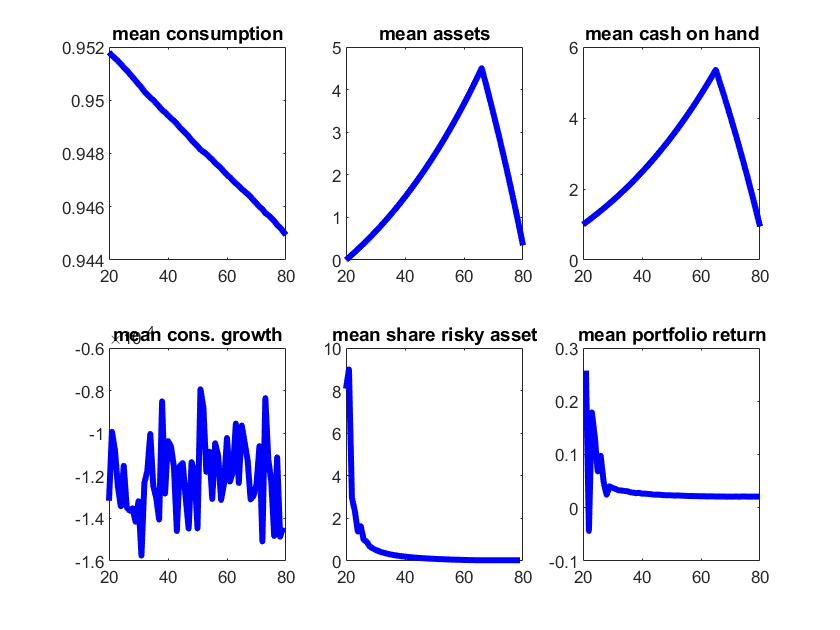
\includegraphics[width = 0.9\textwidth]{PS3/rho0.02tetta150.png}
\\
\textbf{(b) rho = 0.02, tetta=200} \\
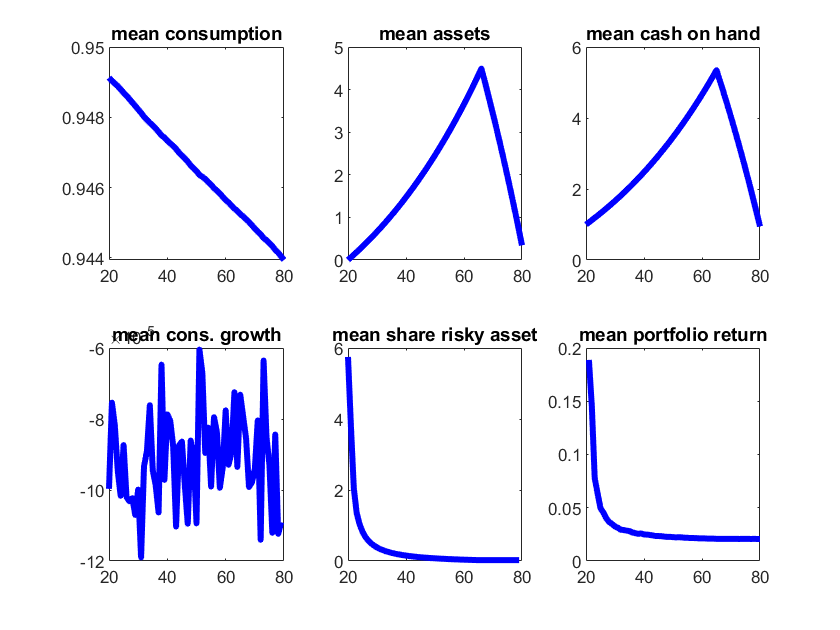
\includegraphics[width = 0.9\textwidth]{PS3/rho0.02tetta200.png}
\\
\textbf{(c) rho = 0.04, tetta=150} \\
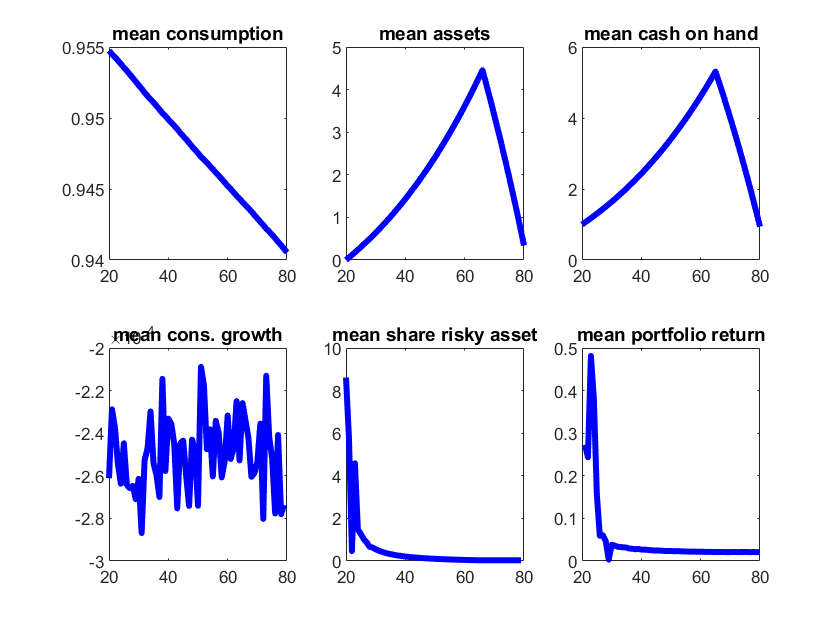
\includegraphics[width = 0.9\textwidth]{PS3/rho0.04tetta150.png}
\\

\section*{Problem 3}
\textbf{Q: Relate the portfolio allocation for the case $\theta = 150$ and $\rho = 0.04$ to the "rule of thumb" advice of a fund manager who suggests to hold $\alpha_j = 1- \frac{j}{100}$ in stocks where $j$ is age.}

Here $\rho$ is chosen to be rather large, leading to a lower $\beta$. This means, that people are more impatient and care relatively more about current consumption (or, expressed differently, care relatively less about future consumption).

Below, there is a graph comparing the recommended share in the risky asset to the estimated model prediction (obviously, this is based on our assumptions about how the returns/ incomes behave).

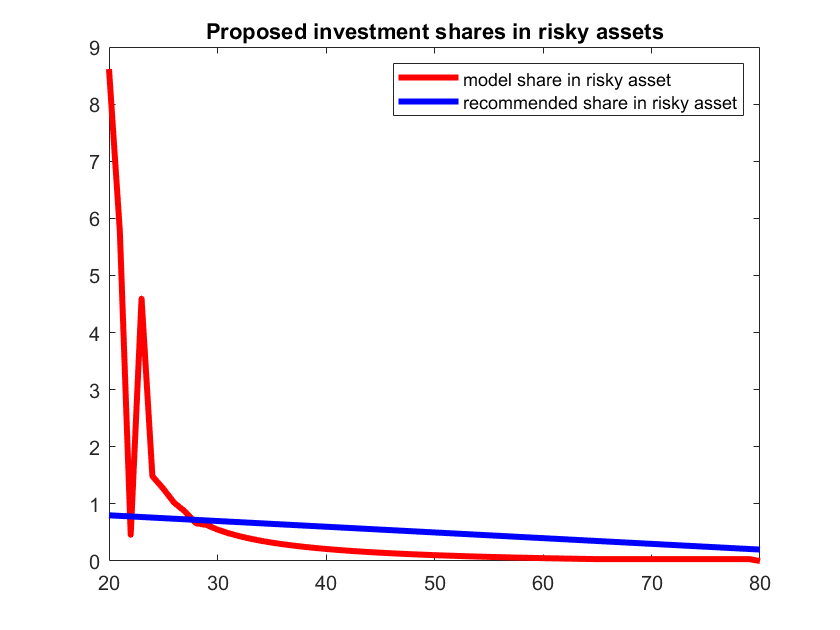
\includegraphics[width = 0.9\textwidth]{PS3/sharesriskyasset.png}
\\
When we run the simulation \textbf{n = 100,000 times} the spike around age 23 becomes less negative\footnote{Note that the kink in some of the variables/ graphs above is because some very drastic shock realizations of the risky asset - it vanishes when we increase the number of simulations.}\\
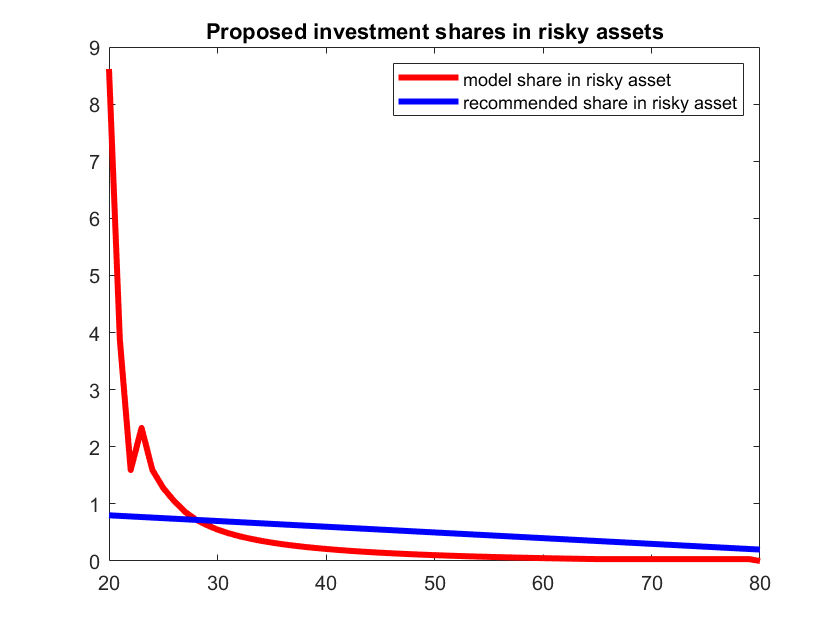
\includegraphics[width = 0.9\textwidth]{PS3/sharesriskyassetns100000.png}
This indicates, that the optimal shares predicted by the model will smooth out when n converges to infinity!

The proposed allocation is linear, which stands in contrast to the model findings. Also, according to the rule of thumb behavior, younger agents should invest in way less risky portfolios than they do in the model. On the other hand, old agents should invest in more risky assets than proposed by the model.


\end{document}